\chapter{Microcontrollers \& the ESP32}\label{ch:mcu}

\begin{tipbox}[When to Read This Chapter]
\textbf{Sprint~3}: Read the ESP32 deep dive, gotchas, and safe GPIO sections before assigning pins at CDR. Print the GPIO pin map table and tape it to your workbench. \textbf{Sprint~4--5}: Return to the communication protocol and firmware best practices sections during integration. \textbf{Related}: Sensors in Chapter~14 (p.\,\pageref{ch:sensors}); driver circuits in Chapter~12 (p.\,\pageref{ch:power}); PCB layout in Chapter~18 (p.\,\pageref{ch:pcb}); debugging in Chapter~20 (p.\,\pageref{ch:debug}).
\end{tipbox}

\vspace{1em}

\section{MCU Fundamentals}
\subsection{What Is a Microcontroller?}
A microcontroller (MCU) integrates a CPU, memory (flash + SRAM), and peripherals (GPIO, ADC, timers, communication) on a single chip. Unlike a microprocessor (Raspberry Pi), an MCU requires no external RAM or storage; it is self-contained and runs bare-metal or RTOS code.

\textbf{Key blocks}: CPU core (executes instructions, 16--600\,MHz), flash memory (stores program, 32\,KB--16\,MB), SRAM (runtime variables, 2\,KB--520\,KB), peripherals (GPIO, ADC, DAC, PWM, timers, watchdog, RTC), communication (UART, SPI, I2C, CAN, Wi-Fi, BLE), and power management (regulators, sleep modes, brown-out detect).

\begin{figure}[htbp]\centering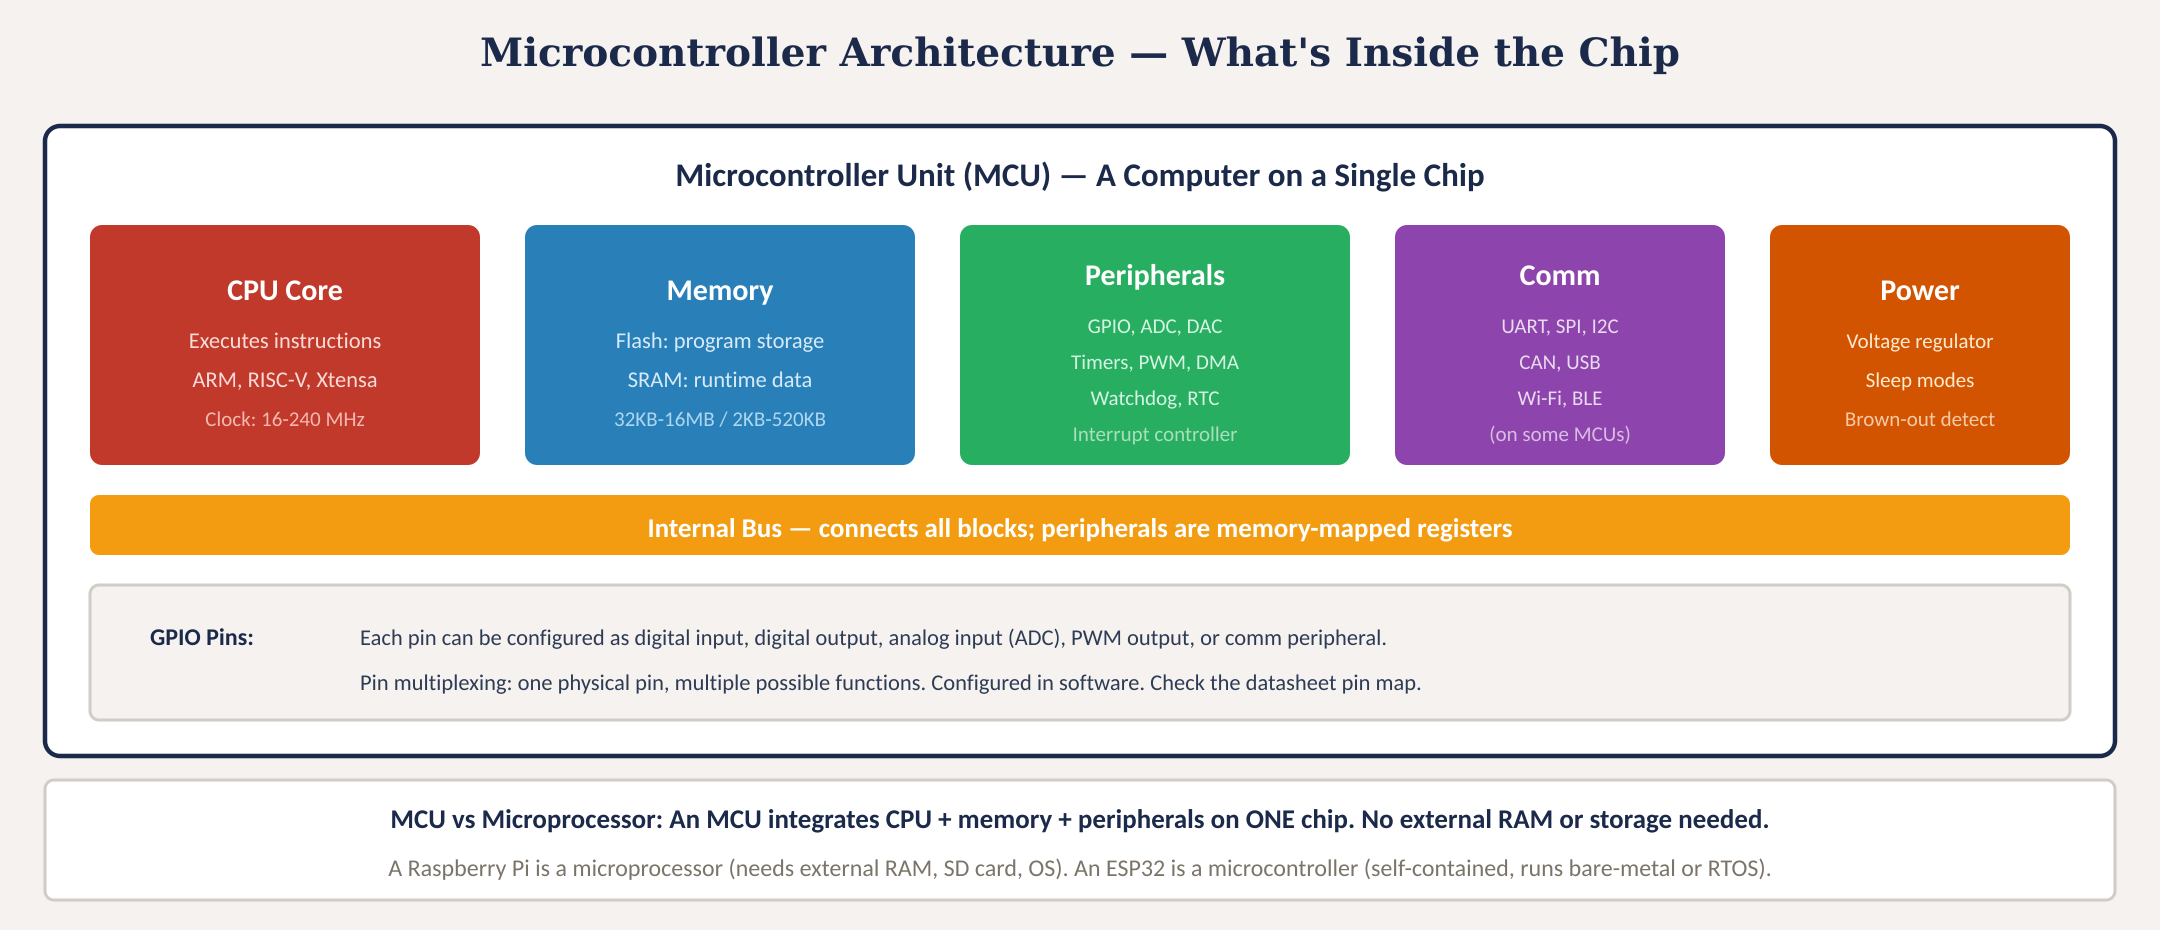
\includegraphics[width=\textwidth]{master_figs/fig_mcu_architecture.png}
\caption{MCU internal architecture: CPU, memory, peripherals, communication, and power on one chip.}\end{figure}

\subsection{MCU Platform Comparison}
\begin{figure}[htbp]\centering% fig_mcu_comparison.tex — Six MCU platforms compared
\begin{tikzpicture}[>=Stealth,
    mcubox/.style={rectangle, rounded corners=3pt, draw=#1, fill=#1!8,
        text width=2.2cm, minimum height=2.6cm, align=center,
        font=\tiny\sffamily, line width=0.7pt, inner sep=4pt},
    mcutitle/.style={font=\scriptsize\sffamily\bfseries, color=#1},
    specrow/.style={font=\tiny\sffamily, color=MinesBlue!80!black},
    recbadge/.style={rectangle, rounded corners=2pt, draw=AccentTeal, fill=AccentTeal!15,
        font=\tiny\sffamily\bfseries, color=AccentTeal, inner sep=2pt}
]

% --- MCU Boxes ---
% Arduino Uno
\node[mcubox=MinesBlue] (m1) at (0,0) {
    ATmega328P\\[2pt]
    16\,MHz, 8-bit\\
    32\,KB flash\\
    2\,KB RAM\\
    14 GPIO, 6 ADC\\
    UART, SPI, I2C\\
    No wireless\\[2pt]
    \textbf{\$3--5}
};
\node[mcutitle=MinesBlue, above=0.15cm of m1] {Arduino Uno};

% Arduino Nano 33 IoT
\node[mcubox=AccentTeal] (m2) at (3.0,0) {
    SAMD21\\[2pt]
    48\,MHz, 32-bit\\
    256\,KB flash\\
    32\,KB RAM\\
    14 GPIO, 8 ADC\\
    UART, SPI, I2C\\
    Wi-Fi + BLE\\[2pt]
    \textbf{\$15--20}
};
\node[mcutitle=AccentTeal, above=0.15cm of m2] {Nano 33 IoT};

% ESP32
\node[mcubox=diagGreen] (m3) at (6.0,0) {
    Xtensa LX6\\[2pt]
    240\,MHz, dual-core\\
    4\,MB flash\\
    520\,KB RAM\\
    34 GPIO, 18 ADC\\
    UART, SPI, I2C, CAN\\
    Wi-Fi + BT + BLE\\[2pt]
    \textbf{\$4--8}
};
\node[mcutitle=diagGreen, above=0.15cm of m3] {ESP32};
\node[recbadge, above=0.55cm of m3] {RECOMMENDED};

% STM32 (Blue Pill)
\node[mcubox=WarnOrange] (m4) at (9.0,0) {
    Cortex-M3\\[2pt]
    72\,MHz, 32-bit\\
    64\,KB flash\\
    20\,KB RAM\\
    37 GPIO, 10 ADC\\
    UART, SPI, I2C, CAN\\
    No wireless\\[2pt]
    \textbf{\$2--5}
};
\node[mcutitle=WarnOrange, above=0.15cm of m4] {STM32 Blue Pill};

% Raspberry Pi Pico
\node[mcubox=diagPurple] (m5) at (12.0,0) {
    RP2040\\[2pt]
    133\,MHz, dual-core\\
    2\,MB flash\\
    264\,KB RAM\\
    26 GPIO, 3 ADC\\
    UART, SPI, I2C\\
    Pico W: Wi-Fi\\[2pt]
    \textbf{\$4--6}
};
\node[mcutitle=diagPurple, above=0.15cm of m5] {RPi Pico};

% Teensy 4.0
\node[mcubox=diagYellow!80!black] (m6) at (15.0,0) {
    Cortex-M7\\[2pt]
    600\,MHz, 32-bit\\
    2\,MB flash\\
    1\,MB RAM\\
    40 GPIO, 14 ADC\\
    UART, SPI, I2C, CAN\\
    No wireless\\[2pt]
    \textbf{\$20--25}
};
\node[mcutitle=diagYellow!80!black, above=0.15cm of m6] {Teensy 4.0};

% Bottom annotation
\node[font=\tiny\sffamily\itshape, color=MinesSilver, text width=14cm, align=center]
    at (7.5,-2.6) {Selection criteria: GPIO count (+20\% margin), protocols needed, processing power, power budget, ecosystem, cost/availability.};

\end{tikzpicture}

\caption{Six MCU platforms compared. ESP32 recommended for MEGN 301.}\end{figure}

\textbf{Selection criteria}: GPIO count (add 20\% margin), communication protocols needed, processing power, power budget (deep sleep current for battery), ecosystem (libraries, community), and cost/availability.

\section{ESP32 Deep Dive}

\begin{tipbox}[ESP32 Variant Landscape]
Espressif has released newer variants of the ESP32 family, including the ESP32-S3 (USB-OTG and vector instructions for AI/ML acceleration), the ESP32-C3 (RISC-V core at lower cost), and the ESP32-C6 (Wi-Fi~6, Thread, and Zigbee support). The ESP32-WROOM-32 remains the recommended platform for MEGN~301 due to its extensive library support, mature documentation, broad community resources, and low cost. Students interested in exploring newer variants for personal or capstone projects can use the same Arduino framework and programming patterns taught in this course.
\end{tipbox}

The ESP32-WROOM-32 is the recommended MCU for MEGN 301 projects: dual-core Xtensa LX6 at 240\,MHz, 520\,KB SRAM, 4\,MB flash, built-in Wi-Fi (802.11 b/g/n) and Bluetooth (Classic + BLE 4.2), 34 GPIO, 18 ADC channels (12-bit), 2 DAC channels (8-bit), 16 PWM channels, 3 UART, 2 SPI, 2 I2C, 1 CAN, 10 capacitive touch pins, deep sleep at $\sim$10\,$\mu$A. Cost: \$4--8 for a DevKit board.

\begin{figure}[htbp]\centering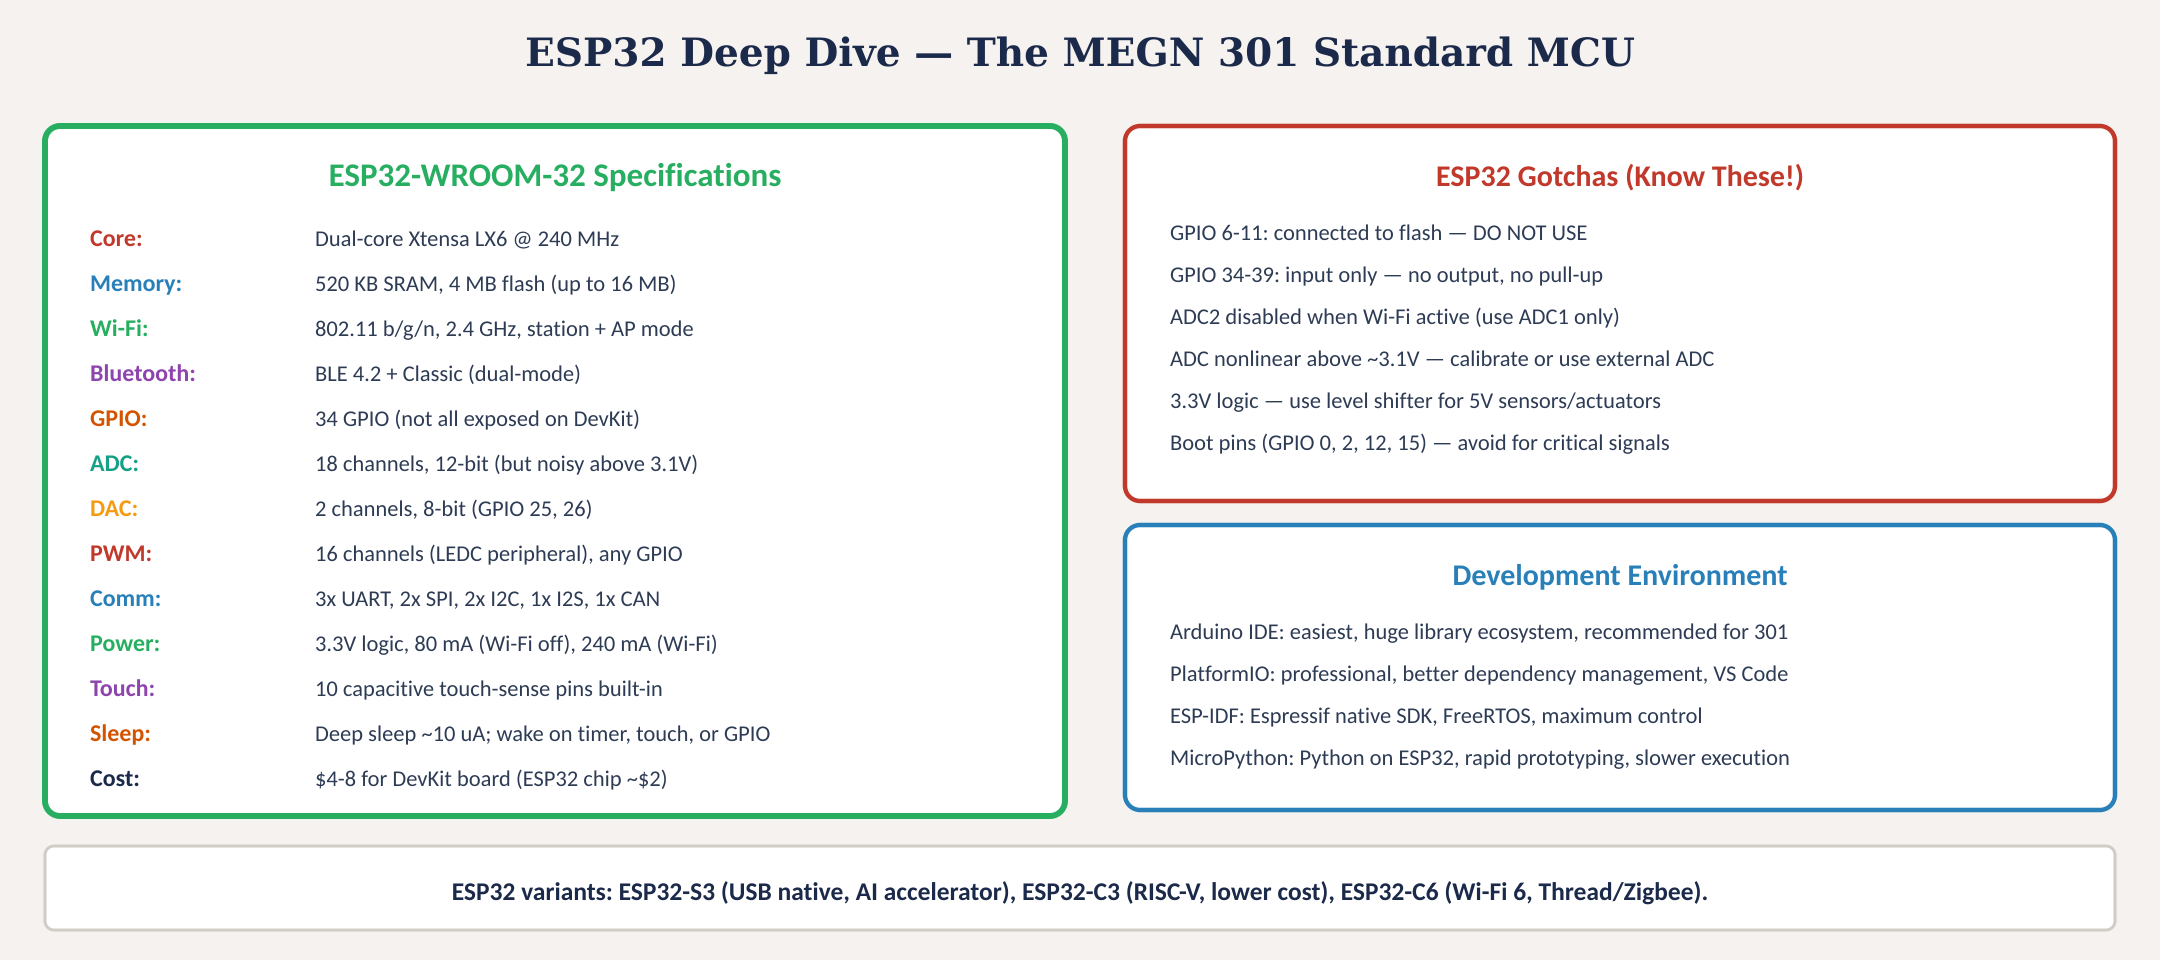
\includegraphics[width=\textwidth]{master_figs/fig_esp32_deep_dive.png}
\caption{ESP32 specifications, gotchas, and development environment.}\end{figure}

\begin{keyconceptbox}[ESP32 Gotchas: Memorize These]
\begin{itemize}[nosep,leftmargin=1.5em]
\item \textbf{GPIO 6--11}: connected to internal flash. DO NOT USE.
\item \textbf{GPIO 34--39}: input only; no output, no internal pull-up.
\item \textbf{ADC2 disabled when Wi-Fi active}: use ADC1 (GPIO 32--39) only.
\item \textbf{ADC nonlinear above $\sim$3.1\,V}: use \texttt{esp\_adc\_cal} library for calibration; design voltage dividers to map sensor output into the 0--2.5\,V linear range rather than using the full 0--3.3\,V span. For precision, use an external ADC (ADS1115, 16-bit, I2C, \$3).
\item \textbf{3.3\,V logic}: use level shifters\index{level shifter} for 5\,V sensors/actuators.
\item \textbf{Boot/strapping pins (0, 2, 5, 12, 15)}: avoid for critical signals; unexpected levels prevent boot.
\end{itemize}
\end{keyconceptbox}

\subsection{Safe GPIO Selection}
\textbf{Safe for any use}: GPIO 4, 13, 14, 16--19, 21--23, 25--27, 32, 33. \textbf{Input only}: GPIO 34, 35, 36 (VP), 39 (VN). \textbf{Boot-sensitive}: GPIO 0, 2, 12, 15 (usable after boot with care). \textbf{Off-limits}: GPIO 6--11 (flash), 1 (TX0), 3 (RX0).

\begin{quickrefbox}[Quick Reference: ESP32 GPIO Pin Map]
\begin{table}[H]\centering\small
\begin{tabularx}{\linewidth}{c c c X}
\toprule
\textbf{GPIO} & \textbf{ADC} & \textbf{Category} & \textbf{Notes} \\
\midrule
4, 13, 14, 16, 17 & --- & Safe & General purpose, any function \\
18, 19, 21, 22, 23 & --- & Safe & SPI default pins (18=SCK, 19=MISO, 23=MOSI) \\
25, 26, 27 & ADC2 & Safe & Also DAC outputs (25=DAC1, 26=DAC2) \\
32, 33 & ADC1 & Safe & Preferred analog inputs (Wi-Fi safe) \\
34, 35, 36, 39 & ADC1 & Input only & No output, no pull-up; use external pull \\
0, 2, 12, 15 & varies & Boot-sensitive & Float or pull as needed; avoid driving at boot \\
6--11 & --- & Off-limits & Internal flash SPI; will crash if used \\
1 (TX0), 3 (RX0) & --- & Serial & USB-serial; avoid for other functions \\
\bottomrule
\end{tabularx}
\end{table}
\end{quickrefbox}

\subsection{Wi-Fi and Bluetooth}
\textbf{Wi-Fi}: Station mode (connect to router), AP mode (create network), or both. ESP-NOW for peer-to-peer without router. \textbf{BLE}: GATT server/client for phone apps; lower power than Classic BT. \textbf{Classic BT}: Serial Port Profile for wireless UART.

\subsection{Power Modes}
Active ($\sim$240\,mA with Wi-Fi), modem sleep ($\sim$20\,mA, radio off), light sleep ($\sim$0.8\,mA, CPU paused), deep sleep ($\sim$10\,$\mu$A, RTC only). Battery sizing example: 2000\,mAh LiPo at active+Wi-Fi = 10 hours; at deep sleep with 1-min wakeups ($\sim$0.5\,mA average) = 166 days.

\section{Communication Protocols}
\begin{figure}[htbp]\centering% fig_mcu_protocols.tex — Six communication protocols comparison
\begin{tikzpicture}[>=Stealth,
    protbox/.style={rectangle, rounded corners=4pt, draw=#1, fill=#1!8,
        text width=2.2cm, minimum height=3.2cm, align=center,
        font=\tiny\sffamily, line width=0.8pt, inner sep=5pt},
    prottitle/.style={font=\scriptsize\sffamily\bfseries, color=#1},
    wireicon/.style={font=\tiny\sffamily\bfseries, color=#1},
    usecase/.style={font=\tiny\sffamily\itshape, color=MinesBlue!60!black, text width=2.2cm, align=center}
]

% --- Protocol boxes ---
% UART
\node[protbox=MinesBlue] (p1) at (0,0) {
    \textbf{2 wires}\\
    TX, RX\\[3pt]
    Point-to-point\\
    9600--115\,k baud\\[3pt]
    Asynchronous\\
    Simple, universal\\[3pt]
    ESP32: 3 ports
};
\node[prottitle=MinesBlue, above=0.15cm of p1] {UART};
\node[usecase, below=0.2cm of p1] {Debug, GPS,\\cellular modules};

% SPI
\node[protbox=AccentTeal] (p2) at (3.0,0) {
    \textbf{4 wires + CS}\\
    SCK, MOSI,\\MISO, CS\\[3pt]
    Bus topology\\
    Up to 80\,MHz\\[3pt]
    Full-duplex\\
    Fastest protocol\\[3pt]
    ESP32: 2 ports
};
\node[prottitle=AccentTeal, above=0.15cm of p2] {SPI};
\node[usecase, below=0.2cm of p2] {Displays, SD cards,\\fast sensors};

% I2C
\node[protbox=WarnOrange] (p3) at (6.0,0) {
    \textbf{2 wires}\\
    SDA, SCL\\[3pt]
    Bus, 127 addr\\
    100--400\,kHz\\[3pt]
    Half-duplex\\
    Needs 4.7\,k pull-ups\\[3pt]
    ESP32: 2 ports
};
\node[prottitle=WarnOrange, above=0.15cm of p3] {I2C};
\node[usecase, below=0.2cm of p3] {Most sensors:\\BME280, MPU6050};

% CAN
\node[protbox=diagPurple] (p4) at (9.0,0) {
    \textbf{2 wires}\\
    CAN\_H, CAN\_L\\[3pt]
    Multi-node\\
    Up to 1\,Mbps\\[3pt]
    Differential\\
    + transceiver IC\\[3pt]
    ESP32: 1 port
};
\node[prottitle=diagPurple, above=0.15cm of p4] {CAN};
\node[usecase, below=0.2cm of p4] {Automotive,\\industrial};

% Wi-Fi
\node[protbox=diagGreen] (p5) at (12.0,0) {
    \textbf{Wireless}\\
    802.11 b/g/n\\[3pt]
    Star (via AP)\\
    Up to 54\,Mbps\\[3pt]
    TCP/UDP/HTTP\\
    High power draw\\[3pt]
    ESP32: built-in
};
\node[prottitle=diagGreen, above=0.15cm of p5] {Wi-Fi};
\node[usecase, below=0.2cm of p5] {IoT, cloud logging,\\OTA updates};

% BLE
\node[protbox=diagYellow!80!black] (p6) at (15.0,0) {
    \textbf{Wireless}\\
    Bluetooth LE 4.2\\[3pt]
    Star / mesh\\
    1--2\,Mbps\\[3pt]
    GATT profiles\\
    Low power\\[3pt]
    ESP32: built-in
};
\node[prottitle=diagYellow!80!black, above=0.15cm of p6] {BLE};
\node[usecase, below=0.2cm of p6] {Phone apps,\\short range};

% Decision rule at bottom
\node[font=\tiny\sffamily\itshape, color=MinesSilver, text width=14cm, align=center]
    at (7.5,-3.3) {Decision rule: I2C for sensors (simple). SPI for displays/SD (fast). UART for debug/GPS. Wi-Fi/BLE for IoT. CAN for automotive.};

\end{tikzpicture}

\caption{Six communication protocols with wire count, speed, topology, and ESP32 support.}\end{figure}

\textbf{UART}: 2 wires, point-to-point, 9600--115200 baud. Debug, GPS, cellular. \textbf{SPI}: 4 wires + CS, bus, up to 80\,MHz. Displays, SD cards, fast sensors. \textbf{I2C}: 2 wires, bus, 100--400\,kHz, 127 addresses. Most sensors (BME280, MPU6050). Needs 4.7\,k$\Omega$ pull-ups. \textbf{CAN}: 2 wires + transceiver, multi-node, 1\,Mbps. Automotive/industrial. \textbf{Wi-Fi/BLE}: wireless IoT.

\begin{tipbox}[Protocol Decision Rule]
I2C for sensors (simple, 2 wires). SPI for displays and SD cards (fast). UART for debug and GPS. Wi-Fi/BLE for IoT connectivity. CAN for automotive.
\end{tipbox}

\section{Firmware and Integration}
\subsection{Firmware Best Practices}
Use \textbf{state machines} (IDLE, READING, TRANSMITTING, SLEEPING). Use \texttt{millis()}-based timing instead of \texttt{delay()}. Use \textbf{interrupts} for hardware events (ISRs must be short; set a flag, process in loop). Enable the \textbf{watchdog timer} for crash recovery. Add a \textbf{heartbeat LED} as a health indicator.

\subsection{System Integration}
\textbf{Power}: 3.3\,V regulated or 5\,V via USB DevKit. Add 10\,$\mu$F + 100\,nF decoupling at MCU power pins. Wi-Fi transmit draws 240\,mA transient; inadequate decoupling causes brown-out resets. \textbf{Level shifting}: BSS138-based modules for I2C/SPI to 5\,V devices. \textbf{I2C}: 4.7\,k$\Omega$ pull-ups to 3.3\,V. \textbf{Analog}: keep wires short, average readings for noise reduction.

\section{Artifact Handoff: What This Chapter Supports}
\begin{table}[htbp]\centering\small
\begin{tabularx}{\textwidth}{l X l}
\toprule
\textbf{Artifact} & \textbf{Description} & \textbf{Key Deliverable For} \\
\midrule
Pin Map & GPIO assignments with function and component & CDR, FDR \\
Firmware Architecture & State machine, ISRs, communication protocols & CDR, FDR \\
Power Mode Plan & Active/sleep duty cycle for battery sizing & CDR (power budget) \\
\bottomrule
\end{tabularx}
\end{table}


\subsection{Development Environment Setup}
\textbf{Arduino IDE} (recommended for MEGN~301): Install Arduino IDE 2.x, add ESP32 board support via Board Manager\footnote{Board Manager URL: \url{https://espressif.github.io/arduino-esp32/package_esp32_index.json}}, select ``ESP32 Dev Module,'' and verify with the Blink example. \textbf{PlatformIO}: more professional, supports version-pinned dependencies and multi-file projects. \textbf{ESP-IDF}: Espressif's native framework; most powerful but steepest learning curve.

\subsection{Common Integration Patterns}
\begin{itemize}[leftmargin=1.5em]
\item \textbf{Sensor polling loop}: read all sensors in \texttt{loop()}, average 3--5 readings, apply calibration, publish to cloud/display. Use \texttt{millis()}-based timing, never \texttt{delay()}.
\item \textbf{Actuator control}: state machine with IDLE, HEATING, COOLING, FAULT states\index{PID controller}. Transitions triggered by sensor thresholds with hysteresis (e.g., turn on at 3\,\degC{}, turn off at 5\,\degC{} to prevent relay chatter).
\item \textbf{Data logging}: write sensor data to SPIFFS/LittleFS with timestamps. Upload batch to cloud on Wi-Fi schedule. Buffer locally if Wi-Fi is unavailable.
\item \textbf{OTA updates}: enable ArduinoOTA for wireless firmware updates during development. Disable in production firmware for security.
\end{itemize}

\subsection{Battery Sizing Worked Example}
GreenShield off-grid: ESP32 wakes every 60\,s for 2\,s of active measurement (80\,mA average during wake, 10\,$\mu$A during sleep). Average current:
\begin{equation}
I_{avg} = \frac{2 \times 80 + 58 \times 0.01}{60} = 2.68\,\text{mA}
\end{equation}
With a 3000\,mAh LiPo: runtime = 3000/2.68 = 1119 hours = 46 days. Adding Wi-Fi transmit (240\,mA for 1\,s every 5 minutes): adds 0.80\,mA average, total 3.48\,mA, runtime = 36 days. Add 30\% margin for battery aging: design for 25 days between charges.


\section{Sensor Interfacing Patterns}

\subsection{Analog Sensors}
Most analog sensors output a voltage proportional to the measured quantity. The ESP32's 12-bit ADC maps 0--3.3\,V to 0--4095 counts. Conversion: $V = \text{count} \times 3.3 / 4095$. Then apply the sensor's transfer function (from datasheet) to convert voltage to engineering units.

\textbf{Common problems and fixes}:
\begin{itemize}[nosep,leftmargin=1.5em]
\item \textbf{Noise}: average 10--50 readings per sample. Use a moving average or median filter in firmware.
\item \textbf{Nonlinearity}: the ESP32 ADC is nonlinear above $\sim$3.1\,V. Use the ESP-IDF calibration API (\texttt{esp\_adc\_cal}) or limit input range to 0--3.0\,V with a voltage divider. For best results: characterize your specific ESP32 module by measuring 10 known voltages (0.0, 0.3, 0.6, \ldots, 3.0\,V from a bench supply) and fitting a polynomial correction in firmware. The 0--2.5\,V range is the most linear; design your voltage divider to map the full sensor range into this window rather than using the full 0--3.3\,V span.
\item \textbf{Offset/gain error}: calibrate against a known reference (multimeter) at two points and apply linear correction: $V_{true} = a \times V_{raw} + b$.
\item \textbf{5\,V sensors}: use a voltage divider or external ADC (ADS1115, 16-bit, I2C, \$3).
\end{itemize}

\subsection{Digital Sensors (I2C)}
Most modern sensors (temperature, humidity, IMU, pressure) use I2C. Basic integration:
\begin{enumerate}[nosep,leftmargin=1.5em]
\item Connect SDA to GPIO~21, SCL to GPIO~22 (ESP32 defaults).
\item Add 4.7\,k$\Omega$ pull-up resistors from SDA and SCL to 3.3\,V. \textbf{One pair per bus}, not per device.
\item Install the sensor's Arduino library via Library Manager.
\item Initialize with \texttt{Wire.begin()} and use the library's \texttt{.read()} methods.
\item If the sensor is not detected: check wiring, verify address with an I2C scanner sketch, check pull-ups with a multimeter (SDA/SCL should read 3.3\,V when idle).
\end{enumerate}

\subsection{Motor and Actuator Control}
\textbf{DC motors}: use \texttt{ledcSetup()} and \texttt{ledcWrite()} for hardware PWM at 20--25\,kHz (above audible range). Never drive a motor directly from a GPIO pin. Always use a driver IC (L298N, BTS7960, DRV8871) or MOSFET with flyback diode.

\textbf{Servo motors}: use the ESP32Servo library. Attach to any PWM-capable GPIO. Standard range: 500--2400\,$\mu$s pulse width at 50\,Hz. Power servos from a separate 5--6\,V supply, not from the ESP32's 3.3\,V rail.

\textbf{Relay control}: drive a relay module's signal input from a GPIO through a 1\,k$\Omega$ resistor. Use optocoupled relay modules to isolate the MCU from relay coil transients.

\section{Debugging and Troubleshooting}

\subsection{Serial Monitor Debugging}
\texttt{Serial.println()} is the primary debugging tool. Best practices:
\begin{itemize}[nosep,leftmargin=1.5em]
\item Print sensor values with labels: \texttt{Serial.print("Temp: "); Serial.println(temp);}
\item Add state machine transitions: \texttt{Serial.println("STATE: HEATING");}
\item Print timestamps: \texttt{Serial.print(millis()); Serial.print(" ms: ");}
\item Remove or conditionally compile debug prints before final deployment (\texttt{\#define DEBUG}).
\end{itemize}

\subsection{Common ESP32 Failure Modes}
\begin{table}[htbp]\centering\small
\begin{tabularx}{\textwidth}{l X X}
\toprule
\textbf{Symptom} & \textbf{Likely Cause} & \textbf{Fix} \\
\midrule
Random resets & Brown-out (insufficient decoupling) & Add 100\,$\mu$F + 100\,nF at regulator output \\
Won't boot & GPIO 0/2/12/15 held at wrong level & Disconnect boot-sensitive pins during upload \\
ADC reads garbage & ADC2 + Wi-Fi conflict, or input $>$3.3\,V & Use ADC1 channels; add voltage divider \\
I2C not detected & Missing pull-ups, wrong address, SDA/SCL swapped & Check with I2C scanner; verify pull-ups \\
Wi-Fi disconnects & Antenna blocked by ground plane or metal & Keep antenna area clear of copper pour \\
Servo jitter & Shared power supply with MCU & Use separate servo power supply \\
\bottomrule
\end{tabularx}
\caption{Common ESP32 failure modes, causes, and fixes.}
\end{table}

\begin{keyconceptbox}[Requirements Mapping: From MCU Specs to Shall-Statements]
MCU capabilities generate system requirements:
\begin{itemize}[nosep,leftmargin=1.5em]
\item ``Read 4 analog sensors'' $\to$ SYS-REQ: The system shall acquire analog data from 4 channels at $\geq$10\,Hz using ADC1 (GPIO 32--35).
\item ``Wireless data logging'' $\to$ SYS-REQ: The system shall transmit sensor data to a cloud server via Wi-Fi at $\geq$1 upload per 5 minutes.
\item ``Battery operation for 30 days'' $\to$ SYS-REQ: The system shall operate from a 3000\,mAh LiPo for $\geq$30 days with a duty cycle of 2\,s active per 60\,s.
\end{itemize}
The battery sizing calculation in this chapter directly verifies the last requirement. Every MCU design choice must trace to a shall-statement.
\end{keyconceptbox}

\section{Microcontroller Fundamentals}
A microcontroller (MCU) is a complete computer on a single chip: processor (CPU), memory (RAM and flash), input/output peripherals, and communication interfaces. Unlike a desktop CPU (which requires external memory, storage, and I/O), the MCU is self-contained and designed for embedded applications where cost, power, and size are constrained.

\subsection{Key Specifications}
\textbf{Clock speed}: determines the instruction execution rate. The ESP32 runs at 240\,MHz (dual core), executing $\sim$240 million simple instructions per second. This is more than adequate for control loops running at 1\,kHz, sensor acquisition, and display updates.

\textbf{Memory}: RAM stores runtime variables (sensor readings, control states, buffers). Flash stores the program (firmware) and constants (calibration tables). The ESP32 has 520\,kB RAM and 4\,MB flash, sufficient for most MEGN~301 projects. If you run out of RAM: optimize data structures, reduce buffer sizes, or use external SPI RAM.

\textbf{GPIO (General Purpose I/O)}: pins that can be configured as digital input, digital output, analog input (ADC), PWM output, or communication interface. The ESP32 has 34 GPIO pins, though some have restrictions (input-only, strapping pins, occupied by flash interface).

\textbf{ADC}: the ESP32's internal ADC is 12-bit with significant nonlinearity and noise ($\pm$50\,LSB at 12-bit). For precision measurement: use an external ADC (ADS1115: 16-bit, I2C, \$3) or the NI~DAQ. The internal ADC is adequate for: battery voltage monitoring, potentiometer reading, and coarse sensor measurement where $\pm$5\% accuracy suffices.

\textbf{Communication interfaces}: UART (serial: 3 ports), SPI (high-speed: 2 ports), I2C (moderate speed: 2 ports). Wi-Fi (802.11b/g/n) and Bluetooth (Classic + BLE) are built-in, enabling wireless data logging, remote monitoring, and over-the-air firmware updates.

\section{ESP32 Pin Planning}
Before writing code, create a pin assignment table mapping every signal to a specific GPIO pin. Constraints to observe:

GPIO 0, 2, 5, 12, 15: strapping pins that affect boot mode. Avoid using for general I/O unless you understand the boot-time implications.

GPIO 34--39: input only (no output capability). Use for analog inputs or digital inputs only.

GPIO 6--11: connected to the internal flash. Do not use.

ADC2 (GPIO 0, 2, 4, 12--15, 25--27): cannot be used for ADC while Wi-Fi is active. Use ADC1 (GPIO 32--39) for analog inputs in Wi-Fi-enabled projects.

\section{Firmware Architecture for Control Systems}
\subsection{Superloop Architecture}
The simplest firmware structure: a single infinite loop that reads sensors, computes control, writes actuators, and updates the display, repeating at a fixed rate:

\begin{verbatim}
void loop() {
  read_sensors();
  compute_pid();
  write_actuators();
  update_display();
  delay_until_next_period();
}
\end{verbatim}

The superloop is adequate for single-rate systems with modest complexity. It fails when: (1) the loop takes longer than the control period (timing violation), (2) different tasks need different rates (sensor at 100\,Hz, display at 10\,Hz, logging at 1\,Hz), or (3) blocking operations (Wi-Fi, SD card write) stall the control loop.

\subsection{Task-Based Architecture (FreeRTOS)}
The ESP32 includes FreeRTOS, a real-time operating system that runs multiple tasks concurrently with priority-based scheduling. Each task has its own stack and runs as if it were the only program. The RTOS scheduler switches between tasks automatically:

High priority: control loop (reads sensor, computes PID, writes actuator). Runs every 10\,ms without interruption.

Medium priority: data logging (writes to SD card). Runs every 1\,s; may be interrupted by the control task.

Low priority: display update and Wi-Fi communication. Runs when higher-priority tasks are idle.

This ensures the control loop always meets its timing deadline, even when lower-priority tasks are slow.

\section{Common ESP32 Pitfalls in MEGN 301}
(1) \textbf{Watchdog timer resets}: the ESP32's watchdog timer resets the system if the main loop (or a FreeRTOS task) does not yield within $\sim$3\,s. Long operations (SD card initialization, Wi-Fi connection) trigger the watchdog. Solution: call \texttt{yield()} or \texttt{vTaskDelay(1)} inside long operations.

(2) \textbf{Power supply noise}: the ESP32's Wi-Fi transmitter draws 120--240\,mA current pulses that cause voltage sag on weak supplies. Symptoms: random resets, ADC reading spikes, Wi-Fi disconnections. Solution: use a dedicated 5\,V supply with $\geq$1\,A capacity and place a 470\,$\mu$F capacitor at the ESP32's 3.3\,V input.

(3) \textbf{GPIO conflicts}: accidentally configuring a strapping pin as output, or using an ADC2 pin while Wi-Fi is active. Symptoms: boot failure, garbage ADC readings. Solution: always check the pin assignment table and the ESP32 datasheet before committing to a pin map.

(4) \textbf{Floating inputs}: unconnected GPIO pins read random noise. If your code checks a button on an unconnected pin, it sees phantom presses. Solution: enable internal pull-up or pull-down resistors on all input pins, or connect external pull-ups/pull-downs.
\begin{keyconceptbox}[Requirements Mapping: Microcontroller Selection]
\textbf{From technical specs to ``shall'' statements:}

The ESP32 ADC has 12-bit resolution on a 0--3.3\,V range (LSB $= 0.8$\,mV) with $\pm$50\,LSB noise ($\pm$40\,mV). For a temperature sensor producing 10\,mV/\degC{}: resolution is $0.8/10 = 0.08$\,\degC{} but noise floor is $40/10 = 4$\,\degC{}. This becomes: ``SYS-ADC-001: The temperature measurement subsystem shall achieve $\pm$0.5\,\degC{} accuracy. \emph{Note: The ESP32 internal ADC cannot meet this requirement. An external ADS1115 (16-bit, $\pm$0.01$\%$ accuracy) shall be used.}''

The ESP32's Wi-Fi transmitter draws 240\,mA peak, causing $\sim$200\,mV sag on a weak 3.3\,V supply. This becomes: ``SYS-PWR-003: The 3.3\,V rail shall maintain $\pm$5\% regulation under Wi-Fi transmit load. \emph{Verification: Test: measure 3.3\,V rail with oscilloscope during Wi-Fi scan.}''
\end{keyconceptbox}
\section{Practice Questions}
\begin{enumerate}[leftmargin=1.5em]
\item Your project requires: 4 analog sensors, 2 PWM motor outputs, I2C temperature sensor, SPI display, Wi-Fi for data logging, and battery operation. Select an MCU platform and justify your choice. Create the pin map.
\item An ESP32 project works on USB power but the MCU resets randomly when running on a 3.7\,V LiPo battery through a 3.3\,V regulator. What is the likely cause? Propose a fix.
\item You need to read a 0--5\,V analog pressure sensor with an ESP32. What problem does this create and how do you solve it?
\item Explain why ADC2 channels should not be used in an ESP32 project that uses Wi-Fi. What happens if you do?
\item A teammate connects a motor driver's PWM input to ESP32 GPIO~8. The ESP32 fails to boot. Why? What GPIO should they use instead?
\item Your I2C temperature sensor (BME280) works perfectly on the bench, but returns \texttt{NaN} after you add a second I2C device (OLED display) to the same bus. Both devices use different I2C addresses. What are the three most likely causes?
\item Design a firmware state machine for the GreenShield frost protection controller. Define all states (at least 4), all transitions, and the conditions that trigger each transition. Include a FAULT state.
\item Your battery-powered sensor node needs to last 60 days on a 2000\,mAh LiPo. The active current is 80\,mA and the deep sleep current is 10\,$\mu$A. What is the maximum duty cycle (active seconds per minute) you can afford?
\end{enumerate}

\subsection{Answers}
\begin{enumerate}[leftmargin=1.5em]
\item ESP32; meets all requirements: 4 ADC1 channels (GPIO 32, 33, 34, 35), 2 PWM (GPIO 25, 26 via LEDC), I2C on GPIO 21 (SDA) / 22 (SCL), SPI display on GPIO 18 (SCK) / 23 (MOSI) / 5 (CS), Wi-Fi built-in, deep sleep for battery life. No other \$4--8 MCU provides Wi-Fi + sufficient ADC + PWM + SPI + I2C simultaneously.
\item Insufficient decoupling. Wi-Fi transmit draws $\sim$240\,mA transient. If the regulator cannot supply this or the decoupling capacitance is too small, the 3.3\,V rail droops below the brown-out threshold ($\sim$2.7\,V) and the ESP32 resets. Fix: add 100\,$\mu$F electrolytic + 100\,nF ceramic at the regulator output. Ensure the regulator can supply $\geq$500\,mA.
\item ESP32 GPIO is 3.3\,V maximum. Applying 5\,V directly will damage the pin. Solution: use a resistive voltage divider (e.g., 10\,k$\Omega$ + 6.8\,k$\Omega$) to scale 0--5\,V to 0--3.0\,V (staying below the 3.1\,V ADC linearity limit), or use an external ADC (ADS1115) with its own voltage reference.
\item ADC2 shares hardware with the Wi-Fi radio. When Wi-Fi is active, the ADC2 peripheral is unavailable. Calling \texttt{analogRead()} on an ADC2 pin returns garbage (random values or zero). Always use ADC1 channels (GPIO 32--39) for analog readings in Wi-Fi projects.
\item GPIO 6--11 are connected to the internal SPI flash that stores the firmware. Any external connection on these pins interferes with flash communication, preventing the bootloader from loading the program. The ESP32 fails to boot or crashes immediately. Use any safe GPIO (4, 13, 14, 16--19, 21--23, 25--27, 32, 33).
\item (1) Duplicate I2C address: despite having different \emph{default} addresses, some modules have configurable addresses that may conflict. Run an I2C scanner to verify both addresses are unique. (2) Pull-up resistor overload: each device may have its own pull-ups on the breakout board. Two sets of 4.7\,k$\Omega$ in parallel = 2.35\,k$\Omega$, which may be too strong for 3.3\,V I2C. Remove the on-board pull-ups from one device. (3) Bus capacitance: the OLED's long ribbon cable adds capacitance, slowing I2C rise times. Try reducing the I2C clock speed from 400\,kHz to 100\,kHz.
\item States: IDLE (monitoring, heater off), HEATING (heater on, monitoring), COOLDOWN (heater off, waiting for hysteresis), FAULT (sensor failure or communication loss). Transitions: IDLE $\to$ HEATING when temp $\leq$ setpoint. HEATING $\to$ COOLDOWN when temp $\geq$ setpoint + hysteresis (e.g., +2\,\degC{}). COOLDOWN $\to$ IDLE when temp stabilizes. Any state $\to$ FAULT when sensor reads out-of-range ($<-40$\,\degC{} or $>85$\,\degC{}) or I2C communication fails 3 consecutive times. FAULT $\to$ IDLE after manual reset via button or remote command.
\item Target runtime: 60 days = 1440 hours. Required average current: $I_{avg} = 2000/1440 = 1.39$\,mA. Let $t_{on}$ = active seconds per 60-second cycle. $I_{avg} = (t_{on} \times 80 + (60 - t_{on}) \times 0.01)/60 = 1.39$. Solving: $t_{on} \times 80 + 0.60 - 0.01 t_{on} = 83.4$. $79.99 t_{on} = 82.8$. $t_{on} = 1.035$\,s. Maximum active time: $\sim$1.0\,s per minute. This is tight; the team should optimize wake time or use a larger battery.
\end{enumerate}



